\documentclass[a4paper,pdftex]{article}

\usepackage{array}
\usepackage{mathtools}
\usepackage{hopsantut}
\usepackage{listings}
\usepackage{todonotes}

\hypersetup{pdfauthor={Robert Braun and Peter Nordin}, pdftitle={Hopsan Tutorial - Getting Started}, pdfsubject={Hopsan Tutorial}}

\lstset{ %
  numbers			=	left,
  numberstyle		=	\scriptsize, % the style that is used for the line-numbers
  backgroundcolor	=\color{yellow!10}
}

\begin{document}
\maketitle{Writing Component Libraries}

\section*{Introduction}
This tutorial will show how to create your own component libraries from C++ by using the HoLC (\underline{Ho}psan \underline{L}ibrary \underline{C}reator) program. \emph{Note!} From Hopsan version 2.13.0 this functionality is also available (and better) inside HopsanGUI. In the first section, the requirements are listed. In the second section, all files in a component library are explained. Finally, creating a library is demonstrated with a step-by-step guide in section three.

\section*{Requirements}
It is strongly recommended to complete the \textit{Getting Started} tutorial before undertaking this one. Some basic knowledge of programming languages are also recommended. 
The following tools are also required:
%
\begin{itemize} %
\itemsep -3pt
\item Hopsan
\item HoLC 
\item Inkscape (optional, for creating component icons)
\end{itemize} %

\section*{Hopsan Component Libraries}
A component library consists of one or more components that can be loaded from Hopsan. It is written in C++ and then compiled to a shared library file (\texttt{.dll} in Windows or \texttt{.so} in Linux). A complete library constists of the files listen below. First, there is a \textit{library description file} in \texttt{.xml} format, which contains basic information about the library. Second, there is a source code file of the library with the \texttt{.cpp} extension.\vspace{10pt}\\
$\mathrm{Component\ Library} \begin{cases}
\mathtt{\textbf{MyLibrary.xml}} \mathrm{\ -\ Library\ description\ file}\\
\mathtt{\textbf{MyLibrary.cpp}} \mathrm{\ -\ Library\ source\ code}\vspace{7pt} \\ 
\begin{rcases}
  \mathtt{\textbf{MyFirstComponent.hpp}} \\
  \mathtt{\textbf{MyFirstComponent.xml}} \\
  \mathtt{\textbf{MyFirstComponent.svg}}
\end{rcases} \mathrm{Component}\vspace{7pt} \\
\begin{rcases}
  \mathtt{\textbf{MySecondComponent.hpp}} \\
  \mathtt{\textbf{MySecondComponent.xml}} \\
  \mathtt{\textbf{MySecondComponent.svg}}
\end{rcases} \mathrm{Component} \\
\end{cases}$
\vspace{10pt}\\
Each component in the library consist of three files. The first one has the \texttt{.hpp} extension, and contains the source code of the component. The second is an \texttt{.xml} file, which contains specifications about the component and its appearance. Finally there is a \texttt{.svg} file, which contains the graphical icon.

\subsection*{Library Description File}
The library description file contains general information, such as name, version and source files.
With this file it is possible to recompile libraries from inside Hopsan.
It also works as a project file for HoLC.
It can for example look like this:

\begin{minipage}{\linewidth}
\begin{lstlisting}[language=xml, basicstyle=\small\ttfamily]
<?xml version="1.0" encoding="UTF-8"?>
<hopsancomponentlibrary xmlversion="0.1" libversion="1" name="LibName">
    <lib>LibName</lib>
    <source>LibName.cpp</source>
    <component>Component1.hpp</component>
    <component>Component2.hpp</component>
    <caf>MyComponent1.xml</caf>
    <caf>MyComponent2.xml</caf>
</hopsancomponentlibrary>
\end{lstlisting}
\end{minipage}

\noindent The first line contains general information about the XML format. It always looks the same. The remaining tags are explained below:

\begin{itemize}
\item \textbf{hopsancomponentlibrary} - Main tag for a component library
\subitem \textbf{xmlversion} - Should always be 0.1 with this XML layout
\subitem \textbf{libversion} - Version of the library (decided by creator)
\subitem \textbf{name} - Name of the library to be shown in Hopsan
\item \textbf{lib} - Base file name of the library file (without prefix, suffix and extension)
\item \textbf{source} - Source file used to compile the library
\item \textbf{component} - Source file for a component in the library
\item \textbf{caf} - Appearance \texttt{.xml} file for a component in the library
\end{itemize}

\subsection*{Library Source File}
The library source file can be viewed as the wrapper file, that takes the source code for each component and puts them together to a library. 
It contains code that is used to register you library components in the HopsanCore, and provides general information about the library for Hopsan.

\begin{minipage}{\linewidth}
\begin{lstlisting}[basicstyle=\footnotesize\ttfamily]
#include "Component1.hpp"
#include "Component2.hpp"

#include "ComponentEssentials.h"
using namespace hopsan;

extern "C" DLLEXPORT void register_contents(ComponentFactory* pComponentFactory, 
                                            NodeFactory* pNodeFactory)
{    
    pComponentFactory->registerCreatorFunction("Component1", Component1::Creator);
    pComponentFactory->registerCreatorFunction("Component2", Component2::Creator);

    HOPSAN_UNUSED(pNodeFactory)
}

extern "C" DLLEXPORT void get_hopsan_info(...)
{
    pHopsanExternalLibInfo->libName = (char*)"LibName";
    pHopsanExternalLibInfo->hopsanCoreVersion = (char*)HOPSANCOREVERSION;
    pHopsanExternalLibInfo->libCompiledDebugRelease = (char*)DEBUGRELEASECOMPILED;
}
\end{lstlisting}
\end{minipage}

\noindent First of all, all component code files must be included. This is shown in lines 1 and 2 in the example below.
Second, each component needs to be registered in the HopsanCore by the "`pComponentFactory->registerCreatorFunction()`", as shown in lines  lines 10 and 11.
The first argument must be a unique \textit{type name} that identifies you component. 
The second argument is the Creator() function, which must exist in each component.
Finally, the \texttt{get\_hopsan\_info()} function must provide a unique \textit{library name}, here called "LibName" at line 18. 
The next two lines should be left as they are.

\subsection*{Component Source Files}
Components are written in C++ files with the .hpp file extension. 
We will now go through the fundamental pars of a component file.\\

\begin{minipage}{\linewidth}
\begin{lstlisting}[basicstyle=\footnotesize\ttfamily]
#ifndef LAMINARORIFICE_H
#define LAMINARORIFICE_H

#include "ComponentEssentials.h"
#include "ComponentUtilities.h"

namespace hopsan {

    class LaminarOrifice : public ComponentQ
    {
    private:
        double *mpP1_p1, *mpP1_q1, *mpP1_c1, *mpP1_Zc1;
        double *mpP2_p2, *mpP2_q2, *mpP2_c2, *mpP2_Zc2, *mpKc;
        Port *mpP1, *mpP2;
       
    public:
        ...
\end{lstlisting}
\end{minipage}

\noindent The first two lines sets a header guard to avoid including the same code twice. 
Then we include the essential functions for the component from \texttt{ComponentEssentials.h}, and all built-in utilities from \texttt{ComponentUtilities.h}.
You may also include other external header files if you wish to use functions from external libraries.\\
\newline
On line 9 the component class is declared. 
We inherit from the \texttt{ComponentQ} class, since this is a Q-type component. 
Similarly we would have used \texttt{ComponentC} for C-type or \texttt{ComponentSignal} for signal type.\\ 
\newline
The first contents in the class is the private variables, which will be persistent in the component. 
In this case we have nine node data pointers and two ports.
A pointer is a variable that points to another variable located somewhere else.
It is used in components to improve performance.
After the private section, the public section begins. 
Public variables and functions can be accessed by the outside world, while private are only allowed to be accessed from functions belonging to the class.

\begin{minipage}{\linewidth}
\begin{lstlisting}[firstnumber=18, basicstyle=\footnotesize\ttfamily]
static Component *Creator()
{
    return new LaminarOrifice();
}
\end{lstlisting}
\end{minipage}

\noindent In the public part we first define a static creator function, which is used to create instances of the component in the simulation core. 
Nothing needs to be changed except the name of the class.

\begin{minipage}{\linewidth}
\begin{lstlisting}[firstnumber=22, basicstyle=\footnotesize\ttfamily]
void configure()
{
    mpP1 = addPowerPort("P1", "NodeHydraulic");
    mpP2 = addPowerPort("P2", "NodeHydraulic");
    addInputVariable("Kc","Coefficient","m^5/Ns", 1.0e-11, &mpIn);
}
\end{lstlisting}
\end{minipage}
\noindent The second function you need to define is the \texttt{configure()} function for the component. 
This function is run every time a new instance of the component is added to the model. 
The function is used to to register ports, input variables, output variables and constants, and to configure default values for persistant variables. 
First we create the ports used for communication with the surrounding components, in this case two hydraulic power ports, see line 24 and 25. 
Then on line 26 we register the restrictor coefficient as an input variable with name, description, unit and default value. 
Input variables can be used either as signal inputs or as parameters.
It is also possible to add constant parameters and output variables using the \texttt{addConstant()} and \texttt{addOutputVariable()} functions.

\begin{minipage}{\linewidth}
\begin{lstlisting}[firstnumber=28, basicstyle=\footnotesize\ttfamily]
void initialize()
{
    mpND_p1 = getSafeNodeDataPtr(mpP1, NodeHydraulic::Pressure);
    mpND_q1 = getSafeNodeDataPtr(mpP1, NodeHydraulic::Flow);
    mpND_c1 = getSafeNodeDataPtr(mpP1, NodeHydraulic::WaveVariable);
    mpND_Zc1 = getSafeNodeDataPtr(mpP1, NodeHydraulic::CharImpedance);

    mpND_p2 = getSafeNodeDataPtr(mpP2, NodeHydraulic::Pressure);
    mpND_q2 = getSafeNodeDataPtr(mpP2, NodeHydraulic::Flow);
    mpND_c2 = getSafeNodeDataPtr(mpP2, NodeHydraulic::WaveVariable);
    mpND_Zc2 = getSafeNodeDataPtr(mpP2, NodeHydraulic::CharImpedance);
}
\end{lstlisting}
\end{minipage}

\noindent The next member function that must be defined is the initialize function. 
This function is run once before each simulation starts. 
As this function is run after connections have been establish you can read or write to/from connected components. 
If needed you can use this information to initialize your component properly. 
This is also the place to allocate additional memory if needed. 
In this case we initialize the component by using the \texttt{getSafeNodeDataPtr()} function to set the node data pointers to point to the variables in the node. 
These lines are always the same for hydraulic nodes, and similar for other node types such as mechanical, pneumatic and electric.

\begin{minipage}{\linewidth}
\begin{lstlisting}[firstnumber=40, basicstyle=\footnotesize\ttfamily]
void simulateOneTimestep()
{
    double p1, q1, c1, Zc1, p2, q2, c2, Zc2;

    //Get variable values from nodes
    c1 = (*mpND_c1);
    Zc1 = (*mpND_Zc1);
    c2 = (*mpND_c2);
    Zc2 = (*mpND_Zc2);
    Kc = (*mpND_Kc);

    //Orifice equations
    q2 = Kc*(c1-c2)/(1.0+Kc*(Zc1+Zc2));
    q1 = -q2;
    p1 = c1 + q1*Zc1;
    p2 = c2 + q2*Zc2;

    //Write new variables to nodes
    (*mpND_p1) = p1;
    (*mpND_q1) = q1;
    (*mpND_p2) = p2;
    (*mpND_q2) = q2;
}
\end{lstlisting}
\end{minipage}

\noindent The next function, \texttt{simulateOneTimestep()}, is the most important function. 
It contains the model equations that are executed each time step. 
We begin on line 42 by creating a local variable for each node data pointer.
The purpose of this is to make the code more readable.
The node data pointers could have been used directly, but this would have been difficult to understand.
Then on line 45-49 we assign all input variables with the values from their respective node data pointer.
Line 52-55 consists of the actual equations. 
In this case we calculate flow and pressure through the orifice from wave variables and impedance in the neighboring C-type components. 
We then end by assigning the output node data pointers with the value of their respective local variable.

\begin{minipage}{\linewidth}
\begin{lstlisting}[firstnumber=63, basicstyle=\footnotesize\ttfamily]
void finalize()
{
      	//Finalize code
}

void deconfigure()
{
    //Deconfigure code
}
\end{lstlisting}
\end{minipage}

\noindent The next function, \texttt{finalize()}, is optional. 
It is only useful if you want some code to be run after each simulation has finished. 
This is usually only needed if you want to free memory that was additionally allocated in the initialize function.\\
\newline
The last function, \texttt{deconfigure()}, is also optional. 
This code is run once the component is deleted. 
Here you can cleanup any memory allocation or similar that you have done in the configure function. 

\subsection*{Component Appearance Files}
Information about the component for the graphical interface, such as icon, port positions and component name, is stored in a \texttt{.xml} file. This file contains information about the component that is not part of the actual simulation code. This information can be changed without the need to recompile the actual component code. A typical appearance file looks like this:

\begin{minipage}{\linewidth}
\begin{lstlisting}[basicstyle=\small\ttfamily]
<?xml version="1.0" encoding="UTF-8"?>
<hopsanobjectappearance version="0.3">
    <modelobject typename="LaminarOrifice" displayname="Orifice" 
                 sourcecode="LaminarOrifice.hpp">
        <icons>
            <icon type="user" path="orifice.svg" 
                  scale="1.0" iconrotation="ON" />
        </icons>
        <help>
            <text>Help Text</text>
            <picture>helpPicture.svg</picture>
            <link>externalHelpDocumentation.pdf</link>
        </help>
        <ports>
            <port x="1,0" y="0.5" a="0" name="P1" visible="true"//>
            <port x="0,0" y="0.5" a="180" name="P2" visible="true"//>
            <port x="0.5" y="0,0" a="270" name="Kc" visible="false"//>
        </ports>
    </modelobject>
</hopsanobjectappearance>
\end{lstlisting}
\end{minipage}

The first line contains basic information about the XML code, and should always look the same. 
A description of the remaining tags follows:

\begin{itemize}
\item \textbf{hopsanobjectappearance} - Main tag for appearance file
\subitem \textbf{version} - Should always be 0.3 with this XML layout
\item \textbf{modelobject} - Main tag for the component
\subitem \textbf{typename} - Unique type name of the component
\subitem \textbf{subtypename} - Specific version of a type name component (optional)
\subitem \textbf{displayname} - Name for the component shown in the graphical interface
\item \textbf{icons} - Contains information about icons. At least one type, user or iso is required
\subitem \textbf{type} - The icon type, user or iso (for ISO 1219 graphics)
\subitem \textbf{path} - Relative path from the \texttt{.xml} file to the \texttt{.svg} icon
\subitem \textbf{scale} - Lets you adjust the scale of the \texttt{.svg} icon (default = 1.0)
\subitem \textbf{iconrotation} - Tells whether or not the icon rotates when the component is rotated
\item \textbf{help} - Allows you to specify help information about the component (optional)
\subitem \textbf{text} - The help text (optional)
\subitem \textbf{picture} - The path to the \texttt{.svg} help picture (optional)
\subitem \textbf{link} - Link to external document relative this \texttt{.xml} file (optional) 
\item \textbf{ports} - Defines the positions and orientations for each port
\subitem \textbf{name} - Name of the port as defined in the code
\subitem \textbf{x} - X-position as fraction of component icon width (0.0 = left, 1.0 = right)
\subitem \textbf{y} - Y-position as fraction of component icon height (0.0 = top, 1.0 = bottom)
\subitem \textbf{a} - Angle of port, 0 = right, 90 = down, 180 = left, 270 = up
\subitem \textbf{visible} - Default visibility state
\end{itemize}

\subsection*{Component Icon Files}
Icons for the graphical interface are stored in the \texttt{.svg} (Scalable Vector Graphics) format. A good and free tool for creating and editing such files is \textit{Inkscape}. If you want to use bitmaps graphics, \texttt{.jpg}, \texttt{.png} or similar formats, such graphics can be embedded in a \texttt{.svg} file.

\section*{Example}
We shall now demonstrate how to build a simple library using HoLC. The library will contain only one simple arithmetic component.

\begin{tutenumerate}
\tutitem{Open HoLC}
Start HoLC by running holc.exe, located in the \texttt{bin} folder under the HoLC directory.

\tutitem{Configure HoLC paths}
First, we must configure HoLC. Click on he options icon:

\icon{0}{gfx/Hopsan-Options.png}{Options}

A component library must be compiled against the version of Hopsan where it shall be used. 
Click on the icon to the right of the "Hopsan Path" field and select your Hopsan installation folder.
It is also necessary to use the correct compiler, depending on if you target the 32-bit or 64-bit version of Hopsan.
Click on the icon next to the compiler path and select the compiler path. 
Compilers are bundled with HoLC and located under the \texttt{ThirdParty} directory.
It should now look something like this:

\frame{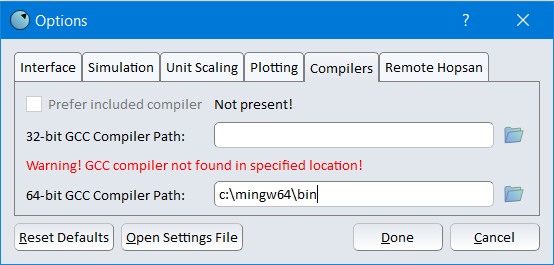
\includegraphics[width=0.7\textwidth]{gfx/writingcomponents/options.png}}

\tutitem{Create a new project}
Now we will create a new empty project. 
First, create an empty folder anywhere on your hard drive.
Click on the \texttt{New Library} icon:

\icon{0}{gfx/Hopsan-New.png}{New Library}

Give the library a name without spaces, for exampe "MyComponentLibrary".
Then click on the folder icon and select the folder you just created.
The dialog should now look like this:

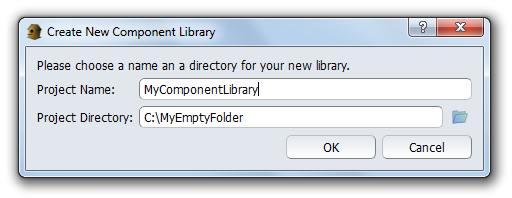
\includegraphics[width=0.7\textwidth]{gfx/writingcomponents/newlibrarydialog.png}.

Click on "OK" to close the dialog.
As you can see, two new files have been created, one \texttt{.xml} file and one .cpp file.

\tutitem{Add a component}
A component library is not very useful without any components.
We now want to create a component that solves the equation $y = A*x+b$.
Click on the \textit{Add New Component} icon:

\icon{0}{gfx/Hopsan-Add.png}{Add New Component}

A component generator dialog appears. 
We need to choose a name.
We also need 2 constants ($A$ and $B$), 1 input variable ($x$) and 1 output variable ($y$).
Enter the following information:

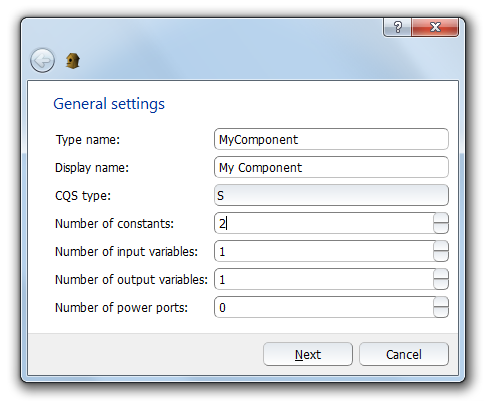
\includegraphics[width=0.65\textwidth]{gfx/writingcomponents/newcomponent1.png}

On the next page you can name the variables and give them default values.
It is also possible to provide units and desriptions.
Name the constants $A$ and $B$, the input variable $x$ and the output variable $y$.
Give $A$ and $B$ the default values 1 and 0.
This means that with default values, $y = x$.

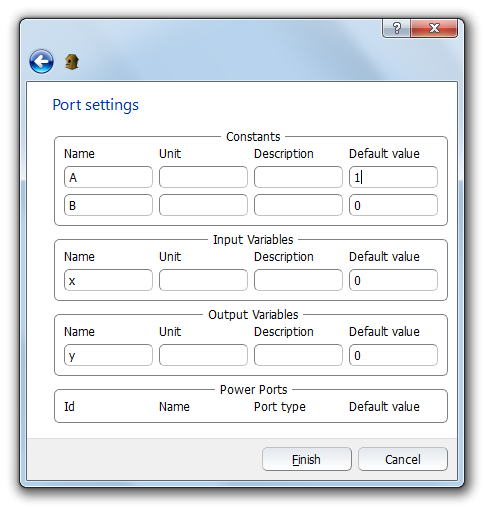
\includegraphics[width=0.65\textwidth]{gfx/writingcomponents/newcomponent2.png}

Ignore units and descriptions for now and click "OK".
Two new files will be created, one \texttt{.hpp} and one \texttt{.xml}.

\tutitem{Write component code}
Now it is time to implement the equation in the component.
Open \texttt{MyComponent.hpp} from the file list.
As you can see, all functions mentioned in the previous chapter has been generated.
In this case we only care about the \texttt{simulateOneTimeStep()} function.
Replace the line "\texttt{//WRITE EQUATIONS HERE}" with the following: "\texttt{y = mA*x+mB;}". Note that in the code, the constants \texttt{A} and \texttt{B} are renamed to \texttt{mA} and \texttt{mB}. This is to indicate that they are \textit{member} variables of the class.
Remember the semicolon!
C++ requires each line to end with a semicolon.\\
\newline\noindent
The component is now ready to be compiled. 
It is possible to modify the port positions in the \texttt{.xml} file, and to create a graphical icon.
Let's ignore that for now.

\tutitem{Compile library}
Click on the compile button in the toolbar:

\icon{0}{gfx/Hopsan-Compile.png}{Compile Library}

The library is now compiled.
Look at the outputs in the terminal at the bottom. 
If everything goes well it should tell use that the compilation was successful. 

\begin{lstlisting}[basicstyle=\small\ttfamily]
Info: Compilation successful.
>> 
\end{lstlisting}

\tutitem{Open library in Hopsan}
Now the library is ready to be loaded from Hopsan.
Start Hopsan, and then click on "Load external library" in the library widget:

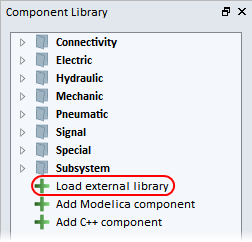
\includegraphics[width=0.4\linewidth]{gfx/writingcomponents/loadlibrary.png}

Browse to the folder you created the library in and choose it.
The component should now be available under the "External Libraries" category.
Build a new model and verify that your own first component works!

\tutitem{Sources of error} %
\vspace{-\baselineskip}
\begin{itemize} %
\item \textbf{Compilation fails in HoLC}\\
This is usually the result of an error in the code. Check the output in HoLC. It can also be caused by tring to compile with 32-bit compiler against 64-bit Hopsan or the other way around.
\item \textbf{Component cannot be loaded in Hopsan}\\
Make sure you are using Hopsan from the same installation directory as you pointed out in HoLC.
\end{itemize}

\end{tutenumerate}
 	
\end{document}
